\section{Introduction}

\subsection{Template}

This is a \gls{latex} thesis template. Uses IEEE-style references\cite{Nescio2024}.

\subsubsection{Figure Example}

Lorem ipsum dolor sit amet, consectetur adipiscing elit, sed do eiusmod tempor incididunt ut labore et dolore magna aliqua.

\begin{figure}[h]
\centering
\label{fig:eximg}
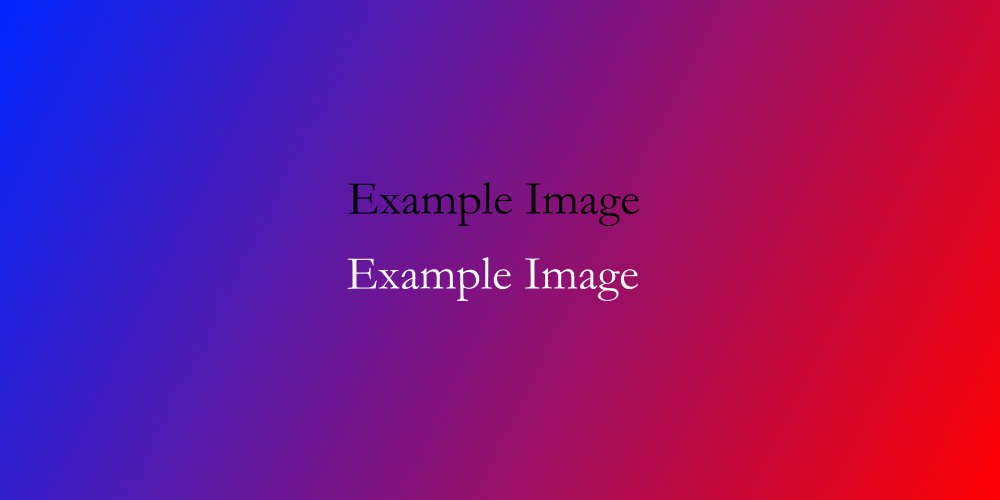
\includegraphics[width=0.7\textwidth]{figures/example/example-image}
\caption{Example of a an image as a figure}
\end{figure}

Lorem ipsum dolor sit amet, consectetur adipiscing elit, sed do eiusmod tempor incididunt ut labore et dolore magna aliqua.

Labels can used to refrence figures, as in this case with figure \ref{fig:eximg}. Lorem ipsum dolor sit amet, consectetur adipiscing elit, sed do eiusmod tempor incididunt ut labore et dolore magna aliqua.

\subsubsection{Maths Example}

An example of a simple equation is:
\begin{equation}
a^2 + b^2 = c^2
\end{equation}
Mathemical expression can also be inlined like \(a^2 + b^2 = c^2\) and ($a$ = 1). Lorem ipsum dolor sit amet, consectetur adipiscing elit, sed do eiusmod tempor incididunt ut labore et dolore magna aliqua.

